% Default 10pt beamer
\documentclass{dt}

\title{There is more to life than SQL!}
\author{Veronika Heimsbakk}

\usepackage{hyperref}

\usepackage{color, colortbl}
\usetikzlibrary{shapes}

\usepackage{tgpagella}
\usepackage[small,euler-digits]{eulervm}
\usepackage{amsmath}

\usepackage{makecell}


\tikzstyle{fargeA}=[fill=red,fill opacity=0.3]
\tikzstyle{fargeB}=[fill=blue,fill opacity=0.3]
\tikzstyle{fargeC}=[fill=green,fill opacity=0.3]

\def\mengdeA{(150:1) circle (1.4cm)}
\def\mengdeB{(30:1) circle (1.4cm)}
\def\mengdeC{(-90:1) circle (1.4cm)}

\newcommand{\dxA}{\draw\mengdeA;}
\newcommand{\dxB}{\draw\mengdeB;}
\newcommand{\dxC}{\draw\mengdeC;}

\newcommand{\fxA}{\fill\mengdeA [fargeA];}
\newcommand{\fxB}{\fill\mengdeB [fargeB];}
\newcommand{\fxC}{\fill\mengdeC [fargeC];}

\newcommand{\clA}{\clip\mengdeA;}
\newcommand{\clB}{\clip\mengdeB;}
\newcommand{\clAB}{\clip\mengdeA\mengdeB;}
\newcommand{\clABC}{\clip\mengdeA\mengdeB\mengdeC;}

\newcommand{\nota}[1]{\node[at={(0,3cm)}]{\ensuremath{#1}}}

\tikzstyle{mikro}=[baseline,scale=0.25,line width=0.5pt]





\begin{document}

{
\setbeamertemplate{footline}{} 
\begin{frame}
\tp{}
\end{frame}
}
\addtocounter{framenumber}{-1}


\begin{frame}
\vspace{20pt}

\presentationframev{img/veronika.jpeg}{
Knowledge Graph Specialist $|$ Data Treehouse


\vspace{2pt}



\includegraphics[width=3cm]{img/dt.png}


\vspace{10pt}

veronika@data-treehouse.com\\
\\
\faGithub{} veleda\\
\faLinkedin{} vheimsbakk\\
\faGlobe{} veronahe.no

\vspace{10pt}

%\includegraphics[width=2cm]{img/cap.jpg}

}
\end{frame}


\begin{frame}
\begin{center}
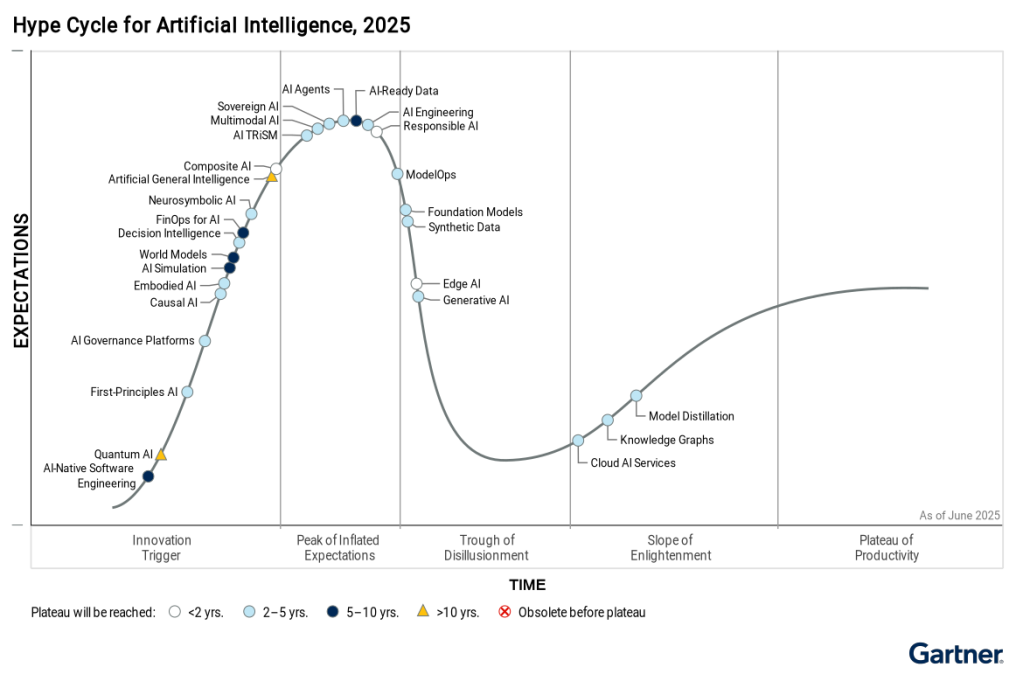
\includegraphics[width=0.8\textwidth]{img/gartner.png}
\end{center}
\end{frame}

\begin{frame}
\begin{center}

\includegraphics[width=0.6\textwidth]{img/graphs.jpg}
\end{center}
\end{frame}

\begin{frame}
\begin{center}
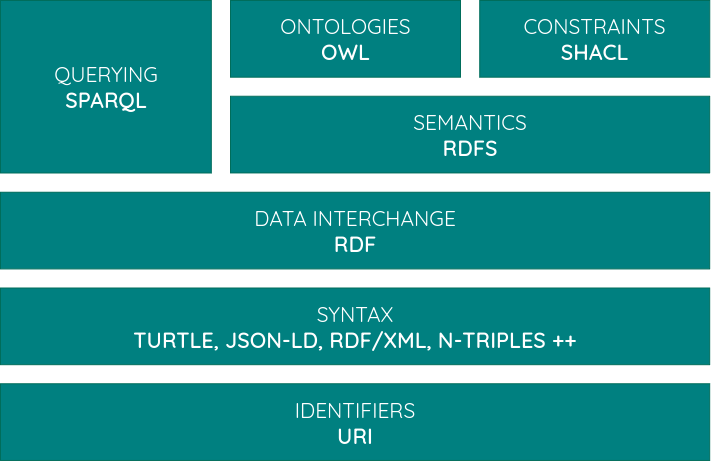
\includegraphics[width=0.6\textwidth]{img/stack-2.png}
\end{center}
\end{frame}

\begin{frame}
\begin{center}
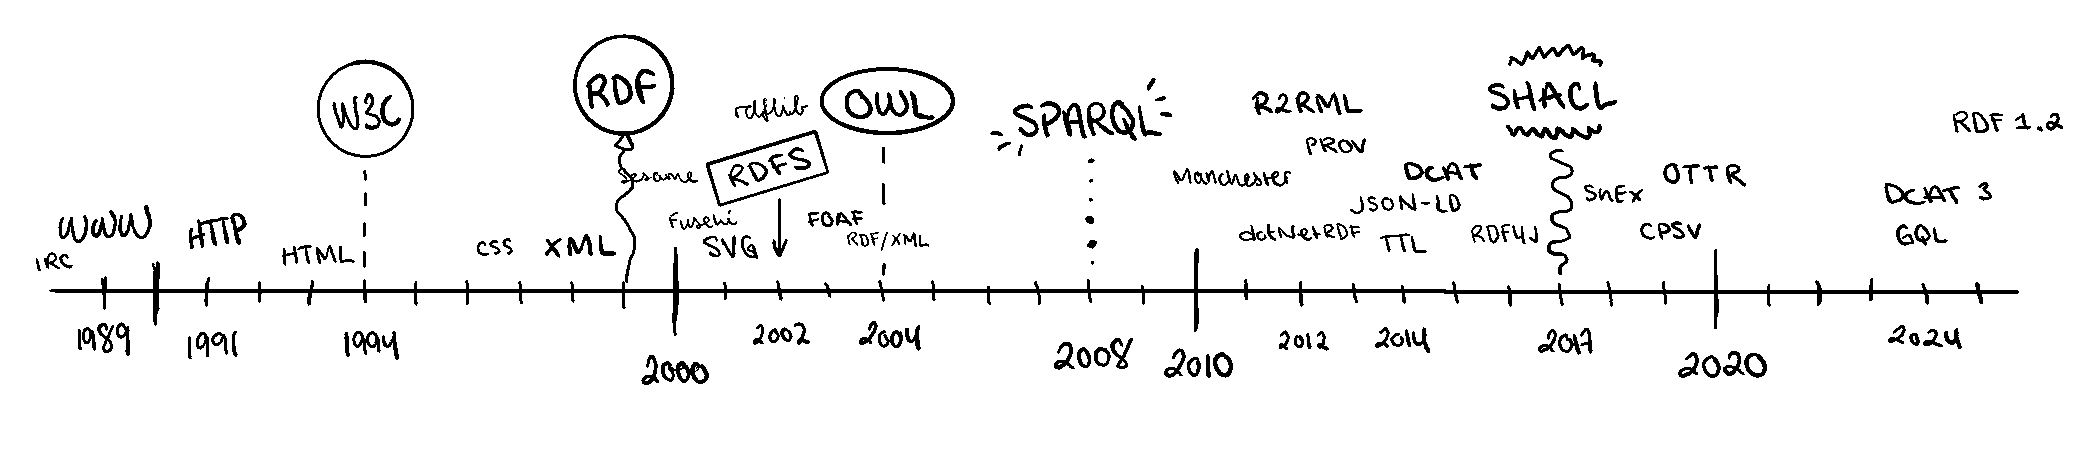
\includegraphics[width=\textwidth]{img/timeline.png}
\end{center}
\end{frame}


\begin{frame}
\Huge{\textbf{RDF}}
\end{frame}


\begin{frame}
Think of data as a \textbf{directed graph}, and that all \textbf{\textit{things}} has a relation to other things.
\end{frame}

\begin{frame}{Terminology}
Think of data as a directed graph, and that all things has a relation to other things.

\begin{itemize}
\item An open standard for representing data as graphs.
\begin{center}

\begin{tikzpicture}
\node[draw=black, ellipse, minimum width=1cm] (1) at (0,0) {};
\node[draw=black, ellipse, minimum width=1cm] (2) at (2,0) {};
\draw[->] (1)--(2);
\end{tikzpicture}
\end{center}
\item Data described as \textbf{triples}.
\item A triple is also called a \textbf{fact} or a \textbf{statement}.
\item The elements of a triple are also called \textbf{resources}.
\begin{center}
\texttt{subject predicate object}
\end{center}
\item Use \textbf{Uniform Resource Identifiers} (URI) as global, unique identifiers.
\end{itemize}
\end{frame}

% URI
\begin{frame}{URI}
\begin{itemize}
\item
\textbf{Only} a \textbf{name}. Does not need to link to anything, URI not URL.
\end{itemize}

\begin{center}
\small{\texttt{scheme:[//[user:password@]host[:port]][/]path[?query][\#fragment]}}
\end{center}

\vspace{10pt}

\textbf{Example}\\
\texttt{http://data.eksempel.no/Kraftverk}

\vspace{10pt}

\begin{tabular}{|l|l|}
\hline
\multicolumn{2}{|c|}{\textbf{URI}}\\
\hline
\textbf{Namespace}&\textbf{Resource name}\\
\hline
\texttt{http://data.eksempel.no/}&\texttt{Kraftverk}\\
\hline
\end{tabular}
\end{frame}

\begin{frame}[fragile]
\begin{code}
\begin{verbatim}
http://data.eksempel.no/Tynna 
  http://www.w3.org/1999/02/22-rdf-syntax-ns#type http://data.eksempel.no/Kraftverk .
\end{verbatim}
\end{code}
\end{frame}

\begin{frame}[fragile]
\begin{code}
\begin{verbatim}
@prefix rdf: <http://www.w3.org/1999/02/22-rdf-syntax-ns#> .
@prefix : <http://data.eksempel.no/> .

:Tynna rdf:type :Kraftverk .
\end{verbatim}
\end{code}
\end{frame}

\begin{frame}[fragile]{Literals and URIs}
\begin{minipage}{0.65\textwidth}
\begin{code}[width=9.25cm]
\begin{verbatim}
@prefix rdf: <http://www.w3.org/1999/02/22-rdf-syntax-ns#> .
@prefix rdfs: <http://www.w3.org/2000/01/rdf-schema#> .
@prefix xsd: <http://www.w3.org/2001/XMLSchema#> .
@prefix : <http://data.eksempel.no/> .

:Tynna a :Kraftverk ;
  rdfs:label "Tynna"@nb, "Tynna"@en ;
  :kommune :Rennebu ;
  :erIDrift true ;
  :iDriftDato "1913-01-01"^^xsd:date ;
  :maksYtelse "0.07"^^xsd:double .
\end{verbatim}
\end{code}
\end{minipage}
\begin{minipage}{0.32\textwidth}
\scalebox{0.8}{
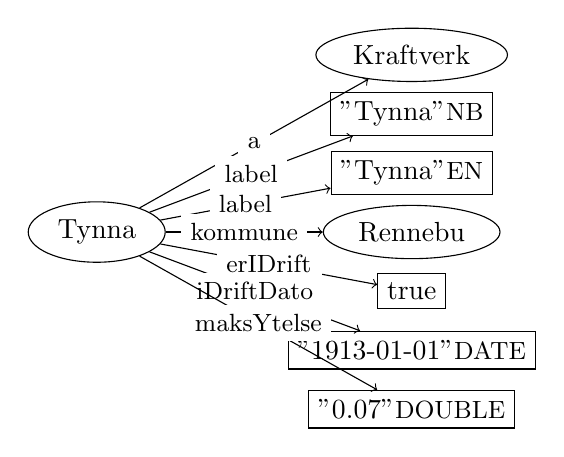
\begin{tikzpicture}
\node[ellipse, draw=black] (1) at (0,-2.25) {Tynna};
\node[ellipse, draw=black] (2) at (4,0) {Kraftverk};
\node[rectangle, draw=black] (3) at (4,-0.75) {"Tynna"\small{NB}};
\node[rectangle, draw=black] (4) at (4,-1.5) {"Tynna"\small{EN}};
\node[ellipse, draw=black] (5) at (4,-2.25) {Rennebu};
\node[rectangle, draw=black] (6) at (4,-3) {true};
\node[rectangle, draw=black] (7) at (4,-3.75) {"1913-01-01"\small{DATE}};
\node[rectangle, draw=black] (8) at (4,-4.5) {"0.07"\small{DOUBLE}};

\draw[->] (1) --node[fill=white]{\small{a}} (2);
\draw[->] (1) --node[fill=white]{\small{label}} (3);
\draw[->] (1) --node[fill=white]{\small{label}} (4);
\draw[->] (1) --node[fill=white]{\small{kommune}} (5);
\draw[->] (1) --node[fill=white]{\small{erIDrift}} (6);
\draw[->] (1) --node[fill=white]{\small{iDriftDato}} (7);
\draw[->] (1) --node[fill=white]{\small{maksYtelse}} (8);
\end{tikzpicture}
}
\end{minipage}

\end{frame}

\begin{frame}[fragile]{Property semantics}
\begin{code}
\begin{verbatim}
@prefix rdf: <http://www.w3.org/1999/02/22-rdf-syntax-ns#> .
@prefix rdfs: <http://www.w3.org/2000/01/rdf-schema#> .
@prefix : <http://data.eksempel.no/> .

:kommune a rdf:Property ;
  rdfs:label "kommune"@nb, "municipality"@en ;
  rdfs:domain :Kraftverk ;
  rdfs:range :Kommune .
\end{verbatim}
\end{code}
\end{frame}

\begin{frame}[fragile]{}
\begin{code}
\begin{verbatim}
@prefix rdf: <http://www.w3.org/1999/02/22-rdf-syntax-ns#> .
@prefix rdfs: <http://www.w3.org/2000/01/rdf-schema#> .
@prefix skos: <http://www.w3.org/2004/02/skos/core#> .
@prefix : <http://data.eksempel.no/> .

:Kraftverk a rdfs:Class ;
  skos:prefLabel "Kraftverk"@nb, "Power station"@en ;
  skos:altLabel "Power plant"@en .

:Vannkraftverk rdfs:subClassOf :Kraftverk ;
  skos:prefLabel "Vannkraftverk"@nb, "Vasskraftverk"@nn, "Hydroelectric power station"@en .

:Mikrovannkraftverk rdfs:subClassOf :Vannkraftverk .

:Vindkraftverk rdfs:subClassOf :Kraftverk .
\end{verbatim}
\end{code}
\end{frame}




\begin{frame}
\Huge{\textbf{DATA}}
\end{frame}

\begin{frame}{}
\begin{center}
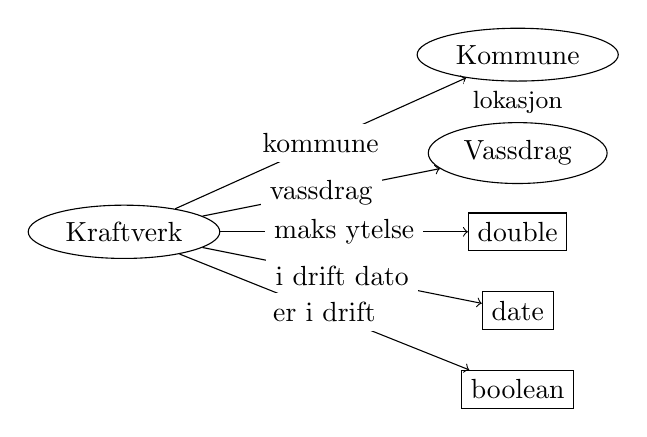
\begin{tikzpicture}
\node[ellipse, draw=black] (1) at (0,-1) {Kraftverk};
\node[ellipse, draw=black] (2) at (5,0) {Vassdrag};
\node[ellipse, draw=black] (3) at (5,1.25) {Kommune};
\node[rectangle, draw=black] (4) at (5,-1) {double};
\node[rectangle, draw=black] (5) at (5,-2) {date};
\node[rectangle, draw=black] (6) at (5,-3) {boolean};

\draw[->] (1) --node[fill=white]{kommune} (3); 
\draw[->] (1) --node[fill=white]{vassdrag} (2);
\draw[->] (1) --node[fill=white]{maks ytelse} (4);  
\draw[->] (1) --node[fill=white]{i drift dato} (5); 
\draw[->] (1) --node[fill=white]{er i drift} (6); 
\draw[->] (2) --node[fill=white]{\small{lokasjon}} (3);
\end{tikzpicture}
\end{center}
\vspace{5pt}
\small{\textbf{NVE Vannkraftverk} \url{https://www.nve.no/energi/energisystem/vannkraft/vannkraftdatabase/}}
\end{frame}

\begin{frame}{}
\begin{center}
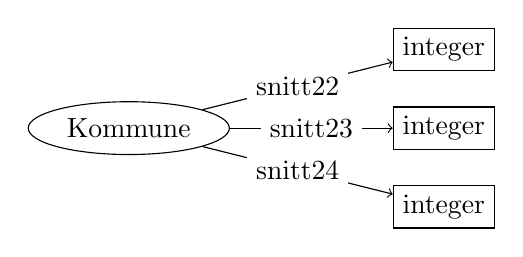
\begin{tikzpicture}
\node[ellipse, draw=black] (3) at (5,1.25) {Kommune};

\node[rectangle, draw=black] (7) at (9,2.25) {integer};
\node[rectangle, draw=black] (8) at (9,1.25) {integer};
\node[rectangle, draw=black] (9) at (9,0.25) {integer};

\draw[->] (3) --node[fill=white]{snitt22} (7); 
\draw[->] (3) --node[fill=white]{snitt23} (8); 
\draw[->] (3) --node[fill=white]{snitt24} (9); 
\end{tikzpicture}
\end{center}

\vspace{5pt}
\small{\textbf{SSB Lønn} \url{https://www.ssb.no/statbank/table/12852/}}
\end{frame}

\begin{frame}{Global, unique identifiers \faHeart{}}
\begin{center}
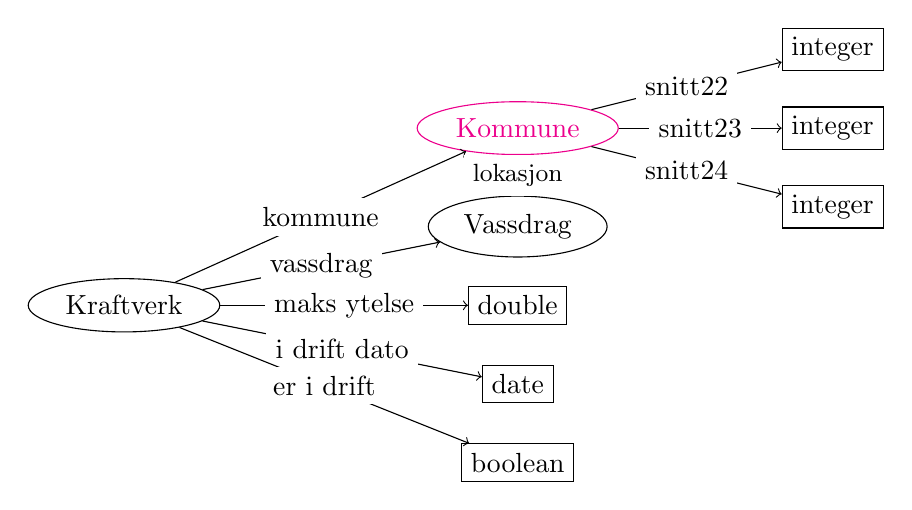
\begin{tikzpicture}
\node[ellipse, draw=black] (1) at (0,-1) {Kraftverk};
\node[ellipse, draw=black] (2) at (5,0) {Vassdrag};
\node[ellipse, draw=magenta, text=magenta] (3) at (5,1.25) {Kommune};
\node[rectangle, draw=black] (4) at (5,-1) {double};
\node[rectangle, draw=black] (5) at (5,-2) {date};
\node[rectangle, draw=black] (6) at (5,-3) {boolean};

\draw[->] (1) --node[fill=white]{kommune} (3); 
\draw[->] (1) --node[fill=white]{vassdrag} (2);
\draw[->] (1) --node[fill=white]{maks ytelse} (4);  
\draw[->] (1) --node[fill=white]{i drift dato} (5); 
\draw[->] (1) --node[fill=white]{er i drift} (6); 
\draw[->] (2) --node[fill=white]{\small{lokasjon}} (3);

\node[rectangle, draw=black] (7) at (9,2.25) {integer};
\node[rectangle, draw=black] (8) at (9,1.25) {integer};
\node[rectangle, draw=black] (9) at (9,0.25) {integer};

\draw[->] (3) --node[fill=white]{snitt22} (7); 
\draw[->] (3) --node[fill=white]{snitt23} (8); 
\draw[->] (3) --node[fill=white]{snitt24} (9); 
\end{tikzpicture}
\end{center}
\end{frame}

\begin{frame}
\Huge{\textbf{ONTOLOGIES}}
\end{frame}

\begin{frame}{Ontology}

\begin{description}
\item[Vocabulary] A collection of words, concepts, terms (and/or RDF resources).
\item[Taxonomy] A classification of the vocabulary.
\item[Ontology] A description of concepts and categories (classes) and their properties, including the
relation between them.
\end{description}

The software I use: Protégé --- \url{https://protege.stanford.edu/}
\end{frame}

\begin{frame}
\begin{minipage}{0.55\textwidth}

\scalebox{0.8}{
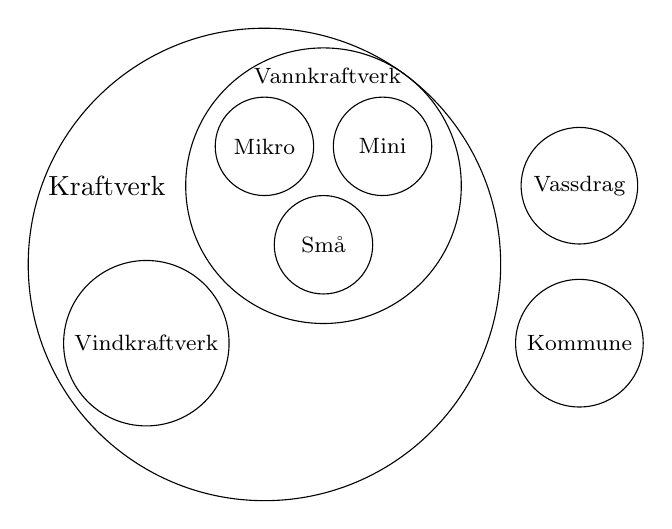
\begin{tikzpicture}
\node[circle, draw=black, minimum width=6cm] (1) at (0,0) {}; 
\node[circle, draw=black, minimum width=3.5cm] (2) at (0.75,1) {}; 
\node[] (2) at (0.8,2.4) {\footnotesize{Vannkraftverk}}; 
\node[] (2) at (-2,1) {{Kraftverk}}; 
\node[circle, draw=black, minimum width=1.25cm] (3) at (0,1.5) {\footnotesize{Mikro}}; 
\node[circle, draw=black, minimum width=1.25cm] (3) at (1.5,1.5) {\footnotesize{Mini}}; 
\node[circle, draw=black, minimum width=1.25cm] (3) at (0.75,0.25) {\footnotesize{Små}}; 
\node[circle, draw=black, minimum width=1.5cm] (4) at (-1.5,-1) {\footnotesize{Vindkraftverk}}; 

\node[circle, draw=black, minimum width=1.25cm] (5) at (4,1) {\footnotesize{Vassdrag}}; 
\node[circle, draw=black, minimum width=1.25cm] (5) at (4,-1) {\footnotesize{Kommune}}; 
\end{tikzpicture}
}


\end{minipage}
\begin{minipage}{0.35\textwidth}
\begin{tabular}{ll}
\textbf{Properties}&\textbf{Datatype}\\
kommune&Kommune (URI)\\
vassdrag&Vassdrag (URI)\\
maks ytelse&double\\
i drift dato&date\\
er i drift&boolean\\
snitt22&integer\\
snitt23&integer\\
snitt24&integer\\
\end{tabular}
\end{minipage}
\end{frame}



\begin{frame}
\Huge{\textbf{MAPPING}}
\end{frame}

\begin{frame}{Resonable Ontology Templates (OTTR)}
\begin{itemize}
\item Mapping language for RDF
\item Open source
\item Developed by academia in Norway, used in industry
\item[\faGlobe{}] \url{https://ottr.xyz/}
\item[\faGithub{}] \url{https://github.com/veleda/ottr-masterclass}
\end{itemize}
\end{frame}

\begin{frame}{tpl}
\begin{center}
\includegraphics[width=0.8\textwidth]{img/xls.png}

\vspace{5pt}

$\downarrow$

\vspace{5pt}

\includegraphics[width=0.3\textwidth]{img/tpl.png}
\end{center}
\end{frame}

\begin{frame}[fragile]{Generate RDF from input through mapping}
\begin{code}
\begin{verbatim}
m = Mapping(tpl)
m.expand(tpl_uri, input_data)
m.write_triples(output, format="turtle")
\end{verbatim}
\end{code}

\vspace{10pt}

Framework for Python: \url{https://datatreehouse.github.io/maplib}

\end{frame}

\begin{frame}
\begin{center}
\begin{tabular}{|l|c|l|}
\hline
\textbf{SQL}&&\textbf{SPARQL}\\
\hline
\makecell[l]{ \texttt{SELECT *} \\ \texttt{FROM A} \\ \texttt{INNER JOIN B} \\ \texttt{ON A.KEY = B.KEY} }&  
\tikz[mikro]{\begin{scope}\clA\clB\fxA\fxB\end{scope}\dxA\dxB\nota{A\cap B}}\hfil&
\makecell[l]{ \texttt{SELECT *} \\ \texttt{WHERE} \\ \texttt{\hspace{2pt} A B}}\\ \hline
\makecell[l]{\texttt{SELECT *} \\ \texttt{FROM A} \\ \texttt{LEFT JOIN B} \\ \texttt{ON A.KEY = B.KEY}}&
  \tikz[mikro]{\fxA\dxA\dxB\nota{A}}\hfil &
\makecell[l]{\texttt{SELECT *} \\ \texttt{WHERE} \\ \texttt{\hspace{2pt} A OPTIONAL \{B\}}}\\ \hline
\makecell[l]{\texttt{SELECT *} \\ \texttt{FROM A} \\ \texttt{LEFT JOIN B} \\ \texttt{ON A.KEY = B.KEY} \\ \texttt{WHERE B.KEY IS NULL}}&
  \tikz[mikro]{\begin{scope}[even odd rule]\clAB\fxA\end{scope}\dxA\dxB\nota{A\setminus B}}\hfil&
\makecell[l]{\texttt{SELECT *} \\ \texttt{WHERE} \\ \texttt{\hspace{2pt} A FILTER NOT EXSISTS \{B\}}}\\ \hline
\makecell[l]{\texttt{SELECT *} \\ \texttt{FROM A} \\ \texttt{OUTER JOIN B} \\ \texttt{ON A.KEY = B.KEY} }&
  \tikz[mikro]{\fxA\fxB\dxA\dxB\nota{A\cup B}}\hfil&
\makecell[l]{\texttt{SELECT *} \\ \texttt{WHERE} \\ \texttt{\hspace{2pt} \{A\} UNION \{B\}}}\\ \hline
\end{tabular}
\end{center}
\end{frame}


\end{document}